% Author Alfredo Sánchez Alberca (asalber@ceu.es)

\section{Descriptive Statistics}
\begin{enumerate}[leftmargin=*]
\item Classify the following variables
\begin{enumerate}
\item Daily hours of exercise.
\item Nationality.
\item Blood pressure.
\item Severity of illness. 
\item Number of sport injuries in a year.
\item Daily calorie intake.
\item Size of clothing.
\item Subjects passed in a course. 
\end{enumerate}

\item \label{soccer-injuries}The number of injuries suffered by the members of a soccer team in a league were
\begin{center}
0 \quad 1 \quad 2 \quad 1 \quad 3 \quad 0 \quad 1 \quad 0 \quad 1 \quad 2 \quad 0 \quad 1 \\
1 \quad 1 \quad 2 \quad 0 \quad 1 \quad 3 \quad 2 \quad 1 \quad 2 \quad 1 \quad 0 \quad 1
\end{center}

\begin{enumerate}
\item Construct the frequency distribution table of the sample.
\item Draw the bar chart of the sample and the polygon.
\item Draw the cumulative frequency bar chart and the polygon. 
\end{enumerate}

\item A survey about the daily number of medicines consumed by people over 70 years, shows the following results:

\begin{center}
3\quad 1\quad 2\quad 2\quad 0\quad 1\quad 4\quad 2\quad 3\quad 5\quad 1\quad 3\quad 2\quad 3\quad 1\quad 4\quad 2\quad 4\quad 3\quad 2 \\
3\quad 5\quad 0\quad 1\quad 2\quad 0\quad 2\quad 3\quad 0\quad 1\quad 1\quad 5\quad 3\quad 4\quad 2\quad 3\quad 0\quad 1\quad 2\quad 3
\end{center} 

\begin{enumerate}
\item Construct the frequency distribution table of the sample.
\item Draw the bar chart of the sample and the polygon.
\item Draw the cumulative relative frequency bar chart and the polygon. 
\end{enumerate}

\item In survey about the dependency of older people, 23 persons over 75 years were asked about the help they need in
daily life. 
The answers were
\begin{center}
B\quad D\quad A\quad B\quad C\quad C\quad B\quad C\quad D\quad E\quad A\quad B\quad C\quad E\quad A\quad B\quad C\quad
D\quad B\quad B\quad A\quad A\quad B 
\end{center}

where the meanings of letters are: 
\begin{enumerate}
\item[A] No help.
\item[B] Help climbing stairs.
\item[C] Help climbing stairs and getting up from a chair or bed.
\item[D] Help climbing stairs, getting up and dressing.
\item[E] Help for almost everything.  
\end{enumerate}

Construct the frequency distribution table and the suitable chart.

\item\label{emergency-service} The number of people treated in the emergency service of a hospital every day of November
was
\begin{center}
15 \quad 23 \quad 12 \quad 10 \quad 28 \quad 7 \quad 12 \quad 17 \quad 20 \quad 21 \quad 18 \quad 13 \quad 11 \quad 12 \quad 26 \\
30 \quad 6 \quad 16 \quad 19 \quad 22 \quad 14 \quad 17 \quad 21 \quad 28 \quad 9 \quad 16 \quad 13 \quad 11 \quad 16 \quad 20
\end{center}

\begin{enumerate}
\item Construct the frequency distribution table of the sample.
\item Draw a suitable chart for the frequency distribution. 
\item Draw a suitable chart for the cumulative frequency distribution.
\end{enumerate}

\item The following frequency distribution table represents the distribution of time (in min) required by people
attended in a medical dispensary. 
\[
\begin{array}{|c|c|c|c|c|}
\hline \mbox{Time} & n_{i} & f_{i} & N_{i} & F_{i}\\
\hline 
\left[ 0,5\right) & 2 &  &  &  \\ 
\hline 
\left[ 5,10\right) &  &  & 8 &  \\ 
\hline 
\left[ 10,15\right) &  & &  & 0.7 \\ 
\hline 
\left[ 15,20\right) & 6 &  &  &\\ 
\hline
\end{array}
\]

\begin{enumerate}
\item Complete the table.
\item Draw the ogive. 
\end{enumerate}

\item Use the data of exercise~\ref{soccer-injuries} to calculate the following statistics and interpret them.
\begin{enumerate}
\item Mean.
\item Median.
\item Mode.
\item Quartiles.
\item Percentile 32.
\end{enumerate}

\itemThe chart below shows the cumulative distribution of the time (in min)
required by 20 students to do an exam.
\begin{center}
\resizebox{0.7\textwidth}{!}{% Created by tikzDevice version 0.9 on 2016-02-01 18:27:14
% !TEX encoding = UTF-8 Unicode
\begin{tikzpicture}[x=1pt,y=1pt]
\definecolor{fillColor}{RGB}{255,255,255}
\path[use as bounding box,fill=fillColor,fill opacity=0.00] (0,0) rectangle (505.89,361.35);
\begin{scope}
\path[clip] ( 49.20, 61.20) rectangle (480.69,312.15);
\definecolor{drawColor}{RGB}{65,105,225}

\path[draw=drawColor,line width= 1.2pt,line join=round,line cap=round] ( 65.18, 70.49) --
	(145.09,102.18) --
	(224.99,123.30) --
	(304.90,172.59) --
	(384.80,264.13) --
	(464.71,302.86);
\definecolor{fillColor}{RGB}{65,105,225}

\path[fill=fillColor] ( 65.18, 70.49) circle (  2.25);

\path[fill=fillColor] (145.09,102.18) circle (  2.25);

\path[fill=fillColor] (224.99,123.30) circle (  2.25);

\path[fill=fillColor] (304.90,172.59) circle (  2.25);

\path[fill=fillColor] (384.80,264.13) circle (  2.25);

\path[fill=fillColor] (464.71,302.86) circle (  2.25);
\end{scope}
\begin{scope}
\path[clip] (  0.00,  0.00) rectangle (505.89,361.35);
\definecolor{drawColor}{RGB}{0,0,0}

\node[text=drawColor,anchor=base,inner sep=0pt, outer sep=0pt, scale=  1.20] at (264.94,332.61) {\bfseries Time required by an exam};

\node[text=drawColor,anchor=base,inner sep=0pt, outer sep=0pt, scale=  1.20] at (264.94, 15.60) {Time (in min)};

\node[text=drawColor,rotate= 90.00,anchor=base,inner sep=0pt, outer sep=0pt, scale=  1.20] at ( 10.80,186.67) {Number of students};
\end{scope}
\begin{scope}
\path[clip] (  0.00,  0.00) rectangle (505.89,361.35);
\definecolor{drawColor}{RGB}{0,0,0}

\path[draw=drawColor,line width= 0.4pt,line join=round,line cap=round] ( 65.18, 61.20) -- (464.71, 61.20);

\path[draw=drawColor,line width= 0.4pt,line join=round,line cap=round] ( 65.18, 61.20) -- ( 65.18, 55.20);

\path[draw=drawColor,line width= 0.4pt,line join=round,line cap=round] (145.09, 61.20) -- (145.09, 55.20);

\path[draw=drawColor,line width= 0.4pt,line join=round,line cap=round] (224.99, 61.20) -- (224.99, 55.20);

\path[draw=drawColor,line width= 0.4pt,line join=round,line cap=round] (304.90, 61.20) -- (304.90, 55.20);

\path[draw=drawColor,line width= 0.4pt,line join=round,line cap=round] (384.80, 61.20) -- (384.80, 55.20);

\path[draw=drawColor,line width= 0.4pt,line join=round,line cap=round] (464.71, 61.20) -- (464.71, 55.20);

\node[text=drawColor,anchor=base,inner sep=0pt, outer sep=0pt, scale=  1.00] at ( 65.18, 39.60) {0};

\node[text=drawColor,anchor=base,inner sep=0pt, outer sep=0pt, scale=  1.00] at (145.09, 39.60) {30};

\node[text=drawColor,anchor=base,inner sep=0pt, outer sep=0pt, scale=  1.00] at (224.99, 39.60) {60};

\node[text=drawColor,anchor=base,inner sep=0pt, outer sep=0pt, scale=  1.00] at (304.90, 39.60) {90};

\node[text=drawColor,anchor=base,inner sep=0pt, outer sep=0pt, scale=  1.00] at (384.80, 39.60) {120};

\node[text=drawColor,anchor=base,inner sep=0pt, outer sep=0pt, scale=  1.00] at (464.71, 39.60) {150};

\path[draw=drawColor,line width= 0.4pt,line join=round,line cap=round] ( 49.20, 70.49) -- ( 49.20,299.33);

\path[draw=drawColor,line width= 0.4pt,line join=round,line cap=round] ( 49.20, 70.49) -- ( 43.20, 70.49);

\path[draw=drawColor,line width= 0.4pt,line join=round,line cap=round] ( 49.20, 88.10) -- ( 43.20, 88.10);

\path[draw=drawColor,line width= 0.4pt,line join=round,line cap=round] ( 49.20,105.70) -- ( 43.20,105.70);

\path[draw=drawColor,line width= 0.4pt,line join=round,line cap=round] ( 49.20,123.30) -- ( 43.20,123.30);

\path[draw=drawColor,line width= 0.4pt,line join=round,line cap=round] ( 49.20,140.91) -- ( 43.20,140.91);

\path[draw=drawColor,line width= 0.4pt,line join=round,line cap=round] ( 49.20,158.51) -- ( 43.20,158.51);

\path[draw=drawColor,line width= 0.4pt,line join=round,line cap=round] ( 49.20,176.11) -- ( 43.20,176.11);

\path[draw=drawColor,line width= 0.4pt,line join=round,line cap=round] ( 49.20,193.72) -- ( 43.20,193.72);

\path[draw=drawColor,line width= 0.4pt,line join=round,line cap=round] ( 49.20,211.32) -- ( 43.20,211.32);

\path[draw=drawColor,line width= 0.4pt,line join=round,line cap=round] ( 49.20,228.92) -- ( 43.20,228.92);

\path[draw=drawColor,line width= 0.4pt,line join=round,line cap=round] ( 49.20,246.53) -- ( 43.20,246.53);

\path[draw=drawColor,line width= 0.4pt,line join=round,line cap=round] ( 49.20,264.13) -- ( 43.20,264.13);

\path[draw=drawColor,line width= 0.4pt,line join=round,line cap=round] ( 49.20,281.73) -- ( 43.20,281.73);

\path[draw=drawColor,line width= 0.4pt,line join=round,line cap=round] ( 49.20,299.33) -- ( 43.20,299.33);

\node[text=drawColor,rotate= 90.00,anchor=base,inner sep=0pt, outer sep=0pt, scale=  1.00] at ( 34.80, 70.49) {0};

\node[text=drawColor,rotate= 90.00,anchor=base,inner sep=0pt, outer sep=0pt, scale=  1.00] at ( 34.80, 88.10) {5};

\node[text=drawColor,rotate= 90.00,anchor=base,inner sep=0pt, outer sep=0pt, scale=  1.00] at ( 34.80,105.70) {10};

\node[text=drawColor,rotate= 90.00,anchor=base,inner sep=0pt, outer sep=0pt, scale=  1.00] at ( 34.80,140.91) {20};

\node[text=drawColor,rotate= 90.00,anchor=base,inner sep=0pt, outer sep=0pt, scale=  1.00] at ( 34.80,176.11) {30};

\node[text=drawColor,rotate= 90.00,anchor=base,inner sep=0pt, outer sep=0pt, scale=  1.00] at ( 34.80,211.32) {40};

\node[text=drawColor,rotate= 90.00,anchor=base,inner sep=0pt, outer sep=0pt, scale=  1.00] at ( 34.80,246.53) {50};

\node[text=drawColor,rotate= 90.00,anchor=base,inner sep=0pt, outer sep=0pt, scale=  1.00] at ( 34.80,281.73) {60};
\end{scope}
\begin{scope}
\path[clip] ( 49.20, 61.20) rectangle (480.69,312.15);
\definecolor{drawColor}{RGB}{190,190,190}

\path[draw=drawColor,line width= 0.4pt,dash pattern=on 1pt off 3pt ,line join=round,line cap=round] ( 49.20, 70.49) -- (480.69, 70.49);

\path[draw=drawColor,line width= 0.4pt,dash pattern=on 1pt off 3pt ,line join=round,line cap=round] ( 49.20, 88.10) -- (480.69, 88.10);

\path[draw=drawColor,line width= 0.4pt,dash pattern=on 1pt off 3pt ,line join=round,line cap=round] ( 49.20,105.70) -- (480.69,105.70);

\path[draw=drawColor,line width= 0.4pt,dash pattern=on 1pt off 3pt ,line join=round,line cap=round] ( 49.20,123.30) -- (480.69,123.30);

\path[draw=drawColor,line width= 0.4pt,dash pattern=on 1pt off 3pt ,line join=round,line cap=round] ( 49.20,140.91) -- (480.69,140.91);

\path[draw=drawColor,line width= 0.4pt,dash pattern=on 1pt off 3pt ,line join=round,line cap=round] ( 49.20,158.51) -- (480.69,158.51);

\path[draw=drawColor,line width= 0.4pt,dash pattern=on 1pt off 3pt ,line join=round,line cap=round] ( 49.20,176.11) -- (480.69,176.11);

\path[draw=drawColor,line width= 0.4pt,dash pattern=on 1pt off 3pt ,line join=round,line cap=round] ( 49.20,193.72) -- (480.69,193.72);

\path[draw=drawColor,line width= 0.4pt,dash pattern=on 1pt off 3pt ,line join=round,line cap=round] ( 49.20,211.32) -- (480.69,211.32);

\path[draw=drawColor,line width= 0.4pt,dash pattern=on 1pt off 3pt ,line join=round,line cap=round] ( 49.20,228.92) -- (480.69,228.92);

\path[draw=drawColor,line width= 0.4pt,dash pattern=on 1pt off 3pt ,line join=round,line cap=round] ( 49.20,246.53) -- (480.69,246.53);

\path[draw=drawColor,line width= 0.4pt,dash pattern=on 1pt off 3pt ,line join=round,line cap=round] ( 49.20,264.13) -- (480.69,264.13);

\path[draw=drawColor,line width= 0.4pt,dash pattern=on 1pt off 3pt ,line join=round,line cap=round] ( 49.20,281.73) -- (480.69,281.73);

\path[draw=drawColor,line width= 0.4pt,dash pattern=on 1pt off 3pt ,line join=round,line cap=round] ( 49.20,299.33) -- (480.69,299.33);
\end{scope}
\end{tikzpicture}
}
\end{center}

\begin{enumerate}
\item A which time have finished half of the students? And 90\% of students?
\item Which percentage of students have finished after 100 minutes?
\item Which is the time that best represent the time required by students in the sample to finish the exam? Is this
value representative or not?
\end{enumerate}

\itemIn a study about the children growth two samples where drawn, one for
newborns and the other for one year old.
The height in cm of children in both samples were 
\begin{center}
\begin{tabular}{rl}
Newborn children: & 51, 50, 51, 53, 49, 50, 53, 50, 47, 50\\
One year old children: & 62, 65, 69, 71, 65, 66, 68, 69
\end{tabular}
\end{center}

In which group is more representative the mean? Justify the answer.

\item To determine the accuracy of a method for measuring hematocrit in blood, the measurement was repeated 8 times on
the same blood sample.
The results in percentage of hematocrit in plasma were
\[
42.2\quad 42.1\quad 41.9\quad 41.8\quad 42\quad 42.1\quad 41.9\quad 42
\]
What do you think about the accuracy of the method?


\item The histogram below shows the frequency distribution of the body mass index (BMI) of a group of people by gender.
\begin{center}
\resizebox{0.6\textwidth}{!}{% Created by tikzDevice version 0.9 on 2016-02-01 19:17:20
% !TEX encoding = UTF-8 Unicode
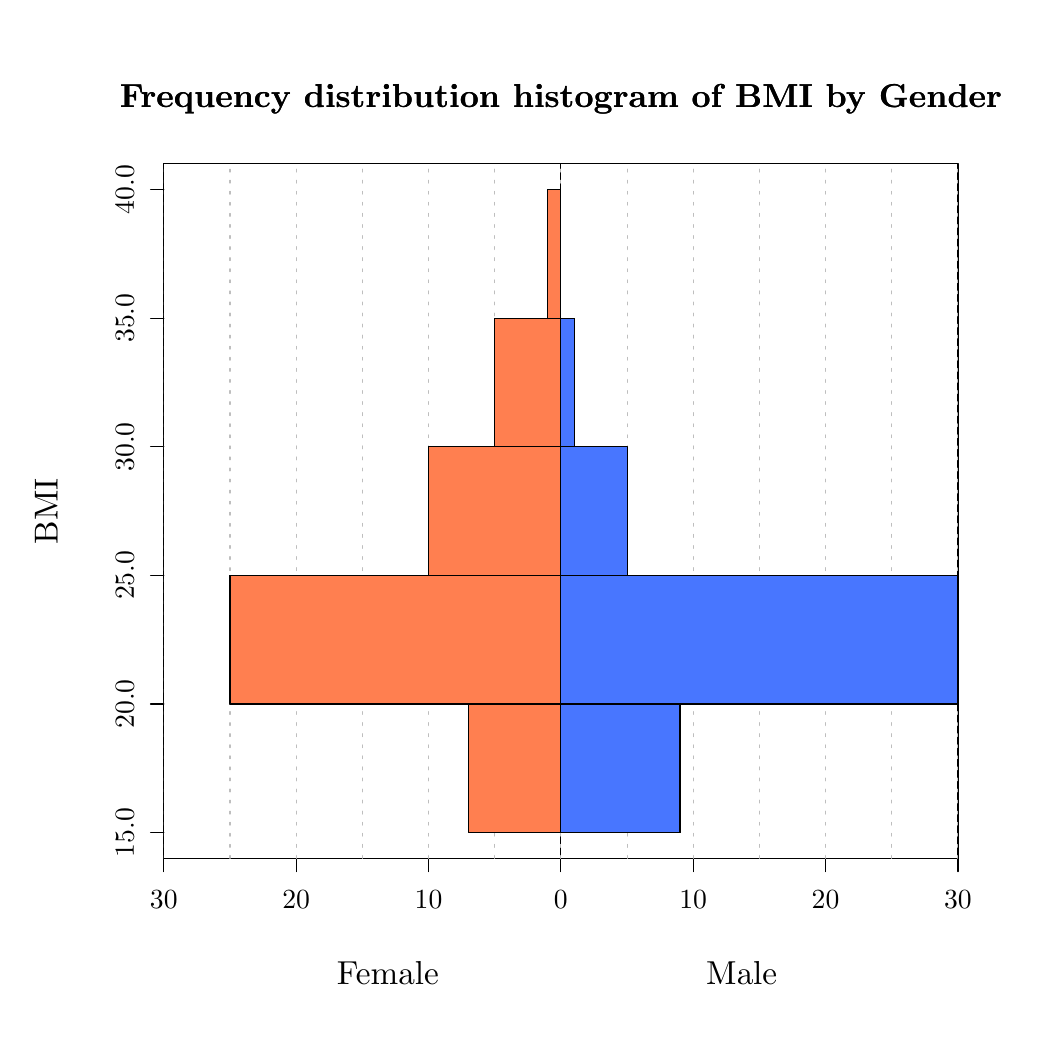
\begin{tikzpicture}[x=1pt,y=1pt]
\definecolor{fillColor}{RGB}{255,255,255}
\path[use as bounding box,fill=fillColor,fill opacity=0.00] (0,0) rectangle (361.35,361.35);
\begin{scope}
\path[clip] (  0.00,  0.00) rectangle (361.35,361.35);
\definecolor{drawColor}{RGB}{0,0,0}

\path[draw=drawColor,line width= 0.4pt,line join=round,line cap=round] (192.68, 70.49) rectangle (159.20,116.97);

\path[draw=drawColor,line width= 0.4pt,line join=round,line cap=round] (192.68,116.97) rectangle ( 73.11,163.44);

\path[draw=drawColor,line width= 0.4pt,line join=round,line cap=round] (192.68,163.44) rectangle (144.85,209.91);

\path[draw=drawColor,line width= 0.4pt,line join=round,line cap=round] (192.68,209.91) rectangle (168.76,256.38);

\path[draw=drawColor,line width= 0.4pt,line join=round,line cap=round] (192.68,256.38) rectangle (187.89,302.86);

\node[text=drawColor,anchor=base,inner sep=0pt, outer sep=0pt, scale=  1.20] at (192.68,332.61) {\bfseries Frequency distribution histogram of BMI by Gender};
\end{scope}
\begin{scope}
\path[clip] (  0.00,  0.00) rectangle (361.35,361.35);
\definecolor{drawColor}{RGB}{0,0,0}

\path[draw=drawColor,line width= 0.4pt,line join=round,line cap=round] (192.68, 70.49) rectangle (235.72,116.97);

\path[draw=drawColor,line width= 0.4pt,line join=round,line cap=round] (192.68,116.97) rectangle (336.15,163.44);

\path[draw=drawColor,line width= 0.4pt,line join=round,line cap=round] (192.68,163.44) rectangle (216.59,209.91);

\path[draw=drawColor,line width= 0.4pt,line join=round,line cap=round] (192.68,209.91) rectangle (197.46,256.38);

\path[draw=drawColor,line width= 0.4pt,line join=round,line cap=round] (192.68,256.38) rectangle (192.68,302.86);

\node[text=drawColor,anchor=base,inner sep=0pt, outer sep=0pt, scale=  1.20] at (192.68,332.61) {\bfseries Frequency distribution histogram of BMI by Gender};
\end{scope}
\begin{scope}
\path[clip] (  0.00,  0.00) rectangle (361.35,361.35);
\definecolor{drawColor}{RGB}{0,0,0}

\path[draw=drawColor,line width= 0.4pt,line join=round,line cap=round] ( 49.20, 61.20) -- (336.15, 61.20);

\path[draw=drawColor,line width= 0.4pt,line join=round,line cap=round] ( 49.20, 61.20) -- ( 49.20, 56.40);

\path[draw=drawColor,line width= 0.4pt,line join=round,line cap=round] ( 97.03, 61.20) -- ( 97.03, 56.40);

\path[draw=drawColor,line width= 0.4pt,line join=round,line cap=round] (144.85, 61.20) -- (144.85, 56.40);

\path[draw=drawColor,line width= 0.4pt,line join=round,line cap=round] (192.68, 61.20) -- (192.68, 56.40);

\path[draw=drawColor,line width= 0.4pt,line join=round,line cap=round] (240.50, 61.20) -- (240.50, 56.40);

\path[draw=drawColor,line width= 0.4pt,line join=round,line cap=round] (288.32, 61.20) -- (288.32, 56.40);

\path[draw=drawColor,line width= 0.4pt,line join=round,line cap=round] (336.15, 61.20) -- (336.15, 56.40);

\node[text=drawColor,anchor=base,inner sep=0pt, outer sep=0pt, scale=  1.00] at ( 49.20, 43.20) {30};

\node[text=drawColor,anchor=base,inner sep=0pt, outer sep=0pt, scale=  1.00] at ( 97.03, 43.20) {20};

\node[text=drawColor,anchor=base,inner sep=0pt, outer sep=0pt, scale=  1.00] at (144.85, 43.20) {10};

\node[text=drawColor,anchor=base,inner sep=0pt, outer sep=0pt, scale=  1.00] at (192.68, 43.20) { 0};

\node[text=drawColor,anchor=base,inner sep=0pt, outer sep=0pt, scale=  1.00] at (240.50, 43.20) {10};

\node[text=drawColor,anchor=base,inner sep=0pt, outer sep=0pt, scale=  1.00] at (288.32, 43.20) {20};

\node[text=drawColor,anchor=base,inner sep=0pt, outer sep=0pt, scale=  1.00] at (336.15, 43.20) {30};

\path[draw=drawColor,line width= 0.4pt,line join=round,line cap=round] ( 49.20, 70.49) -- ( 49.20,302.86);

\path[draw=drawColor,line width= 0.4pt,line join=round,line cap=round] ( 49.20, 70.49) -- ( 44.40, 70.49);

\path[draw=drawColor,line width= 0.4pt,line join=round,line cap=round] ( 49.20,116.97) -- ( 44.40,116.97);

\path[draw=drawColor,line width= 0.4pt,line join=round,line cap=round] ( 49.20,163.44) -- ( 44.40,163.44);

\path[draw=drawColor,line width= 0.4pt,line join=round,line cap=round] ( 49.20,209.91) -- ( 44.40,209.91);

\path[draw=drawColor,line width= 0.4pt,line join=round,line cap=round] ( 49.20,256.38) -- ( 44.40,256.38);

\path[draw=drawColor,line width= 0.4pt,line join=round,line cap=round] ( 49.20,302.86) -- ( 44.40,302.86);

\node[text=drawColor,rotate= 90.00,anchor=base,inner sep=0pt, outer sep=0pt, scale=  1.00] at ( 38.40, 70.49) {15.0};

\node[text=drawColor,rotate= 90.00,anchor=base,inner sep=0pt, outer sep=0pt, scale=  1.00] at ( 38.40,116.97) {20.0};

\node[text=drawColor,rotate= 90.00,anchor=base,inner sep=0pt, outer sep=0pt, scale=  1.00] at ( 38.40,163.44) {25.0};

\node[text=drawColor,rotate= 90.00,anchor=base,inner sep=0pt, outer sep=0pt, scale=  1.00] at ( 38.40,209.91) {30.0};

\node[text=drawColor,rotate= 90.00,anchor=base,inner sep=0pt, outer sep=0pt, scale=  1.00] at ( 38.40,256.38) {35.0};

\node[text=drawColor,rotate= 90.00,anchor=base,inner sep=0pt, outer sep=0pt, scale=  1.00] at ( 38.40,302.86) {40.0};
\end{scope}
\begin{scope}
\path[clip] (  0.00,  0.00) rectangle (361.35,361.35);
\definecolor{drawColor}{RGB}{0,0,0}

\node[text=drawColor,anchor=base,inner sep=0pt, outer sep=0pt, scale=  1.20] at (130.14, 15.60) {Female};

\node[text=drawColor,anchor=base east,inner sep=0pt, outer sep=0pt, scale=  1.20] at (270.83, 15.60) {Male};

\node[text=drawColor,rotate= 90.00,anchor=base,inner sep=0pt, outer sep=0pt, scale=  1.20] at ( 10.80,186.67) {BMI};
\end{scope}
\begin{scope}
\path[clip] ( 49.20, 61.20) rectangle (336.15,312.15);
\definecolor{drawColor}{RGB}{0,0,0}

\path[draw=drawColor,line width= 0.4pt,line join=round,line cap=round] (192.68, 61.20) -- (192.68,312.15);
\end{scope}
\begin{scope}
\path[clip] (  0.00,  0.00) rectangle (361.35,361.35);
\definecolor{drawColor}{RGB}{0,0,0}

\path[draw=drawColor,line width= 0.4pt,line join=round,line cap=round] ( 49.20, 61.20) --
	(336.15, 61.20) --
	(336.15,312.15) --
	( 49.20,312.15) --
	( 49.20, 61.20);
\end{scope}
\begin{scope}
\path[clip] ( 49.20, 61.20) rectangle (336.15,312.15);
\definecolor{drawColor}{RGB}{190,190,190}

\path[draw=drawColor,line width= 0.4pt,dash pattern=on 1pt off 3pt ,line join=round,line cap=round] (  1.38, 61.20) -- (  1.38,312.15);

\path[draw=drawColor,line width= 0.4pt,dash pattern=on 1pt off 3pt ,line join=round,line cap=round] ( 25.29, 61.20) -- ( 25.29,312.15);

\path[draw=drawColor,line width= 0.4pt,dash pattern=on 1pt off 3pt ,line join=round,line cap=round] ( 49.20, 61.20) -- ( 49.20,312.15);

\path[draw=drawColor,line width= 0.4pt,dash pattern=on 1pt off 3pt ,line join=round,line cap=round] ( 73.11, 61.20) -- ( 73.11,312.15);

\path[draw=drawColor,line width= 0.4pt,dash pattern=on 1pt off 3pt ,line join=round,line cap=round] ( 97.03, 61.20) -- ( 97.03,312.15);

\path[draw=drawColor,line width= 0.4pt,dash pattern=on 1pt off 3pt ,line join=round,line cap=round] (120.94, 61.20) -- (120.94,312.15);

\path[draw=drawColor,line width= 0.4pt,dash pattern=on 1pt off 3pt ,line join=round,line cap=round] (144.85, 61.20) -- (144.85,312.15);

\path[draw=drawColor,line width= 0.4pt,dash pattern=on 1pt off 3pt ,line join=round,line cap=round] (168.76, 61.20) -- (168.76,312.15);

\path[draw=drawColor,line width= 0.4pt,dash pattern=on 1pt off 3pt ,line join=round,line cap=round] (192.68, 61.20) -- (192.68,312.15);

\path[draw=drawColor,line width= 0.4pt,dash pattern=on 1pt off 3pt ,line join=round,line cap=round] (216.59, 61.20) -- (216.59,312.15);

\path[draw=drawColor,line width= 0.4pt,dash pattern=on 1pt off 3pt ,line join=round,line cap=round] (240.50, 61.20) -- (240.50,312.15);

\path[draw=drawColor,line width= 0.4pt,dash pattern=on 1pt off 3pt ,line join=round,line cap=round] (264.41, 61.20) -- (264.41,312.15);

\path[draw=drawColor,line width= 0.4pt,dash pattern=on 1pt off 3pt ,line join=round,line cap=round] (288.32, 61.20) -- (288.32,312.15);

\path[draw=drawColor,line width= 0.4pt,dash pattern=on 1pt off 3pt ,line join=round,line cap=round] (312.24, 61.20) -- (312.24,312.15);

\path[draw=drawColor,line width= 0.4pt,dash pattern=on 1pt off 3pt ,line join=round,line cap=round] (336.15, 61.20) -- (336.15,312.15);

\path[draw=drawColor,line width= 0.4pt,dash pattern=on 1pt off 3pt ,line join=round,line cap=round] (360.06, 61.20) -- (360.06,312.15);
\end{scope}
\begin{scope}
\path[clip] (  0.00,  0.00) rectangle (361.35,361.35);
\definecolor{drawColor}{RGB}{0,0,0}
\definecolor{fillColor}{RGB}{255,127,80}

\path[draw=drawColor,line width= 0.4pt,line join=round,line cap=round,fill=fillColor] (192.68, 70.49) rectangle (159.20,116.97);

\path[draw=drawColor,line width= 0.4pt,line join=round,line cap=round,fill=fillColor] (192.68,116.97) rectangle ( 73.11,163.44);

\path[draw=drawColor,line width= 0.4pt,line join=round,line cap=round,fill=fillColor] (192.68,163.44) rectangle (144.85,209.91);

\path[draw=drawColor,line width= 0.4pt,line join=round,line cap=round,fill=fillColor] (192.68,209.91) rectangle (168.76,256.38);

\path[draw=drawColor,line width= 0.4pt,line join=round,line cap=round,fill=fillColor] (192.68,256.38) rectangle (187.89,302.86);
\definecolor{fillColor}{RGB}{72,118,255}

\path[draw=drawColor,line width= 0.4pt,line join=round,line cap=round,fill=fillColor] (192.68, 70.49) rectangle (235.72,116.97);

\path[draw=drawColor,line width= 0.4pt,line join=round,line cap=round,fill=fillColor] (192.68,116.97) rectangle (336.15,163.44);

\path[draw=drawColor,line width= 0.4pt,line join=round,line cap=round,fill=fillColor] (192.68,163.44) rectangle (216.59,209.91);

\path[draw=drawColor,line width= 0.4pt,line join=round,line cap=round,fill=fillColor] (192.68,209.91) rectangle (197.46,256.38);

\path[draw=drawColor,line width= 0.4pt,line join=round,line cap=round,fill=fillColor] (192.68,256.38) rectangle (192.68,302.86);
\end{scope}
\end{tikzpicture}
}
\end{center} 

\begin{enumerate}
\item Draw the pie chart for the gender.
\item In which group is more representative the mean of the BMI?
\item Calculate the mean for the whole sample.
\end{enumerate}
Use the following sums\\
Males: $\sum x_i=1002$ kg/m$^2$ \quad $\sum x_i^2 = 22781$ kg$^2$/m$^4$ \\
Females: $\sum x_i=1160$ kg/m$^2$ \quad $\sum x_i^2 = 29050$ kg$^2$/m$^4$ 

\item The following table represents the frequency distribution of the yearly uses of a health insurance in a sample of
clients of a insurance company.

\begin{center}
\begin{tabular}{lrrrrrrr}
\toprule
Uses: & 0 & 1 & 2 & 3 & 4 & 5 & 7 \\
Clients: & 4 & 8 & 6 & 3 & 2 & 1 & 1\\
\bottomrule
\end{tabular}
\end{center}

Draw the box plot. How is the symmetry of the distribution?


\item The box plots below correspond to the age of a sample of people by marital status.
\begin{center}
\resizebox{0.6\textwidth}{!}{% Created by tikzDevice version 0.9 on 2016-02-01 20:49:53
% !TEX encoding = UTF-8 Unicode
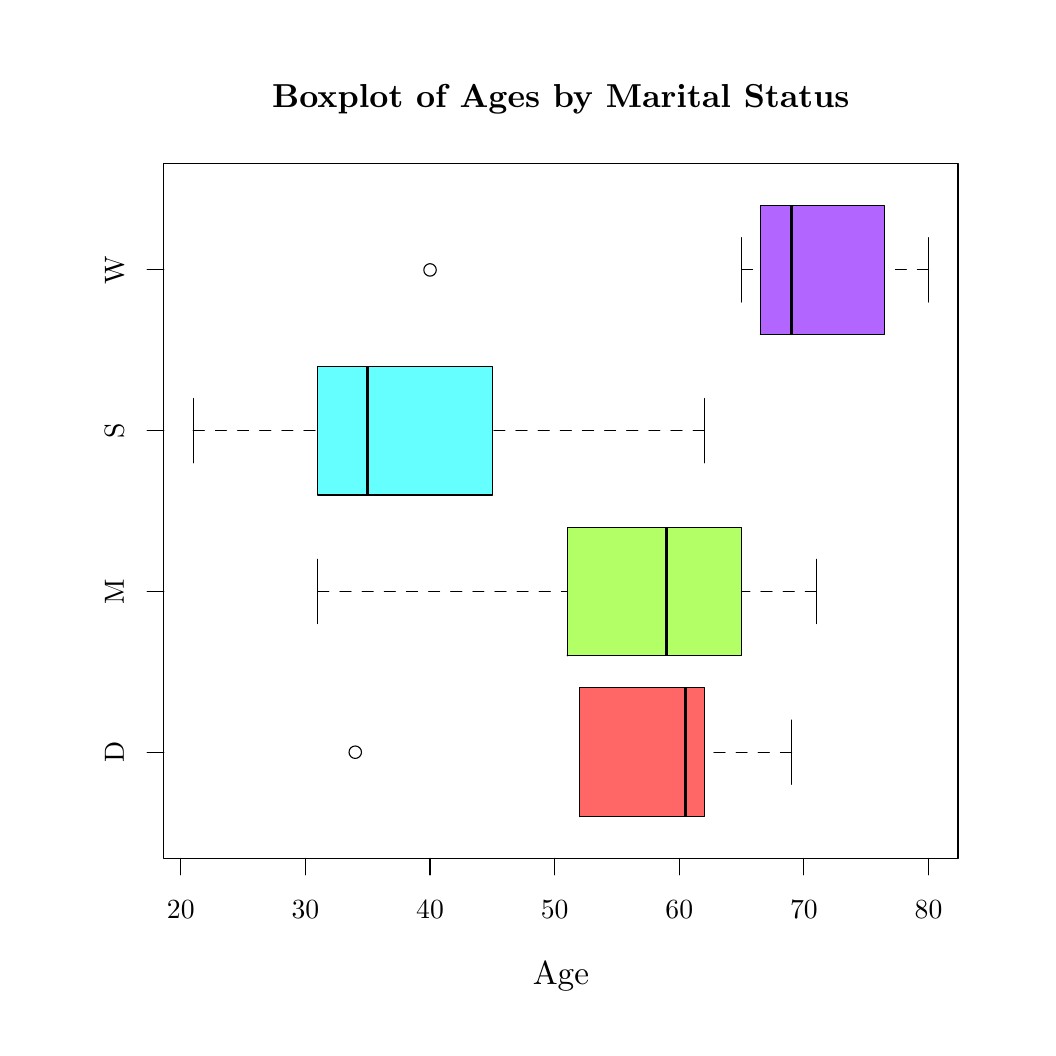
\begin{tikzpicture}[x=1pt,y=1pt]
\definecolor{fillColor}{RGB}{255,255,255}
\path[use as bounding box,fill=fillColor,fill opacity=0.00] (0,0) rectangle (361.35,361.35);
\begin{scope}
\path[clip] ( 49.20, 61.20) rectangle (336.15,312.15);
\definecolor{fillColor}{RGB}{255,102,102}

\path[fill=fillColor] (199.43, 76.30) --
	(199.43,122.78) --
	(244.46,122.78) --
	(244.46, 76.30) --
	cycle;
\definecolor{drawColor}{RGB}{0,0,0}

\path[draw=drawColor,line width= 1.2pt,line join=round] (237.71, 76.30) -- (237.71,122.78);

\path[draw=drawColor,line width= 0.4pt,dash pattern=on 4pt off 4pt ,line join=round,line cap=round] (199.43, 99.54) -- (199.43, 99.54);

\path[draw=drawColor,line width= 0.4pt,dash pattern=on 4pt off 4pt ,line join=round,line cap=round] (275.99, 99.54) -- (244.46, 99.54);

\path[draw=drawColor,line width= 0.4pt,line join=round,line cap=round] (199.43, 87.92) -- (199.43,111.16);

\path[draw=drawColor,line width= 0.4pt,line join=round,line cap=round] (275.99, 87.92) -- (275.99,111.16);

\path[draw=drawColor,line width= 0.4pt,line join=round,line cap=round] (199.43, 76.30) --
	(199.43,122.78) --
	(244.46,122.78) --
	(244.46, 76.30) --
	(199.43, 76.30);

\path[draw=drawColor,line width= 0.4pt,line join=round,line cap=round] (118.37, 99.54) circle (  2.25);
\definecolor{fillColor}{RGB}{179,255,102}

\path[fill=fillColor] (194.93,134.39) --
	(194.93,180.87) --
	(257.97,180.87) --
	(257.97,134.39) --
	cycle;

\path[draw=drawColor,line width= 1.2pt,line join=round] (230.95,134.39) -- (230.95,180.87);

\path[draw=drawColor,line width= 0.4pt,dash pattern=on 4pt off 4pt ,line join=round,line cap=round] (104.86,157.63) -- (194.93,157.63);

\path[draw=drawColor,line width= 0.4pt,dash pattern=on 4pt off 4pt ,line join=round,line cap=round] (284.99,157.63) -- (257.97,157.63);

\path[draw=drawColor,line width= 0.4pt,line join=round,line cap=round] (104.86,146.01) -- (104.86,169.25);

\path[draw=drawColor,line width= 0.4pt,line join=round,line cap=round] (284.99,146.01) -- (284.99,169.25);

\path[draw=drawColor,line width= 0.4pt,line join=round,line cap=round] (194.93,134.39) --
	(194.93,180.87) --
	(257.97,180.87) --
	(257.97,134.39) --
	(194.93,134.39);
\definecolor{fillColor}{RGB}{102,255,255}

\path[fill=fillColor] (104.86,192.48) --
	(104.86,238.96) --
	(167.91,238.96) --
	(167.91,192.48) --
	cycle;

\path[draw=drawColor,line width= 1.2pt,line join=round] (122.87,192.48) -- (122.87,238.96);

\path[draw=drawColor,line width= 0.4pt,dash pattern=on 4pt off 4pt ,line join=round,line cap=round] ( 59.83,215.72) -- (104.86,215.72);

\path[draw=drawColor,line width= 0.4pt,dash pattern=on 4pt off 4pt ,line join=round,line cap=round] (244.46,215.72) -- (167.91,215.72);

\path[draw=drawColor,line width= 0.4pt,line join=round,line cap=round] ( 59.83,204.10) -- ( 59.83,227.34);

\path[draw=drawColor,line width= 0.4pt,line join=round,line cap=round] (244.46,204.10) -- (244.46,227.34);

\path[draw=drawColor,line width= 0.4pt,line join=round,line cap=round] (104.86,192.48) --
	(104.86,238.96) --
	(167.91,238.96) --
	(167.91,192.48) --
	(104.86,192.48);
\definecolor{fillColor}{RGB}{179,102,255}

\path[fill=fillColor] (264.73,250.57) --
	(264.73,297.05) --
	(309.76,297.05) --
	(309.76,250.57) --
	cycle;

\path[draw=drawColor,line width= 1.2pt,line join=round] (275.99,250.57) -- (275.99,297.05);

\path[draw=drawColor,line width= 0.4pt,dash pattern=on 4pt off 4pt ,line join=round,line cap=round] (257.97,273.81) -- (264.73,273.81);

\path[draw=drawColor,line width= 0.4pt,dash pattern=on 4pt off 4pt ,line join=round,line cap=round] (325.52,273.81) -- (309.76,273.81);

\path[draw=drawColor,line width= 0.4pt,line join=round,line cap=round] (257.97,262.19) -- (257.97,285.43);

\path[draw=drawColor,line width= 0.4pt,line join=round,line cap=round] (325.52,262.19) -- (325.52,285.43);

\path[draw=drawColor,line width= 0.4pt,line join=round,line cap=round] (264.73,250.57) --
	(264.73,297.05) --
	(309.76,297.05) --
	(309.76,250.57) --
	(264.73,250.57);

\path[draw=drawColor,line width= 0.4pt,line join=round,line cap=round] (145.39,273.81) circle (  2.25);
\end{scope}
\begin{scope}
\path[clip] (  0.00,  0.00) rectangle (361.35,361.35);
\definecolor{drawColor}{RGB}{0,0,0}

\path[draw=drawColor,line width= 0.4pt,line join=round,line cap=round] ( 49.20, 99.54) -- ( 49.20,273.81);

\path[draw=drawColor,line width= 0.4pt,line join=round,line cap=round] ( 49.20, 99.54) -- ( 43.20, 99.54);

\path[draw=drawColor,line width= 0.4pt,line join=round,line cap=round] ( 49.20,157.63) -- ( 43.20,157.63);

\path[draw=drawColor,line width= 0.4pt,line join=round,line cap=round] ( 49.20,215.72) -- ( 43.20,215.72);

\path[draw=drawColor,line width= 0.4pt,line join=round,line cap=round] ( 49.20,273.81) -- ( 43.20,273.81);

\node[text=drawColor,rotate= 90.00,anchor=base,inner sep=0pt, outer sep=0pt, scale=  1.00] at ( 34.80, 99.54) {D};

\node[text=drawColor,rotate= 90.00,anchor=base,inner sep=0pt, outer sep=0pt, scale=  1.00] at ( 34.80,157.63) {M};

\node[text=drawColor,rotate= 90.00,anchor=base,inner sep=0pt, outer sep=0pt, scale=  1.00] at ( 34.80,215.72) {S};

\node[text=drawColor,rotate= 90.00,anchor=base,inner sep=0pt, outer sep=0pt, scale=  1.00] at ( 34.80,273.81) {W};

\path[draw=drawColor,line width= 0.4pt,line join=round,line cap=round] ( 55.32, 61.20) -- (325.52, 61.20);

\path[draw=drawColor,line width= 0.4pt,line join=round,line cap=round] ( 55.32, 61.20) -- ( 55.32, 55.20);

\path[draw=drawColor,line width= 0.4pt,line join=round,line cap=round] (100.36, 61.20) -- (100.36, 55.20);

\path[draw=drawColor,line width= 0.4pt,line join=round,line cap=round] (145.39, 61.20) -- (145.39, 55.20);

\path[draw=drawColor,line width= 0.4pt,line join=round,line cap=round] (190.42, 61.20) -- (190.42, 55.20);

\path[draw=drawColor,line width= 0.4pt,line join=round,line cap=round] (235.46, 61.20) -- (235.46, 55.20);

\path[draw=drawColor,line width= 0.4pt,line join=round,line cap=round] (280.49, 61.20) -- (280.49, 55.20);

\path[draw=drawColor,line width= 0.4pt,line join=round,line cap=round] (325.52, 61.20) -- (325.52, 55.20);

\node[text=drawColor,anchor=base,inner sep=0pt, outer sep=0pt, scale=  1.00] at ( 55.32, 39.60) {20};

\node[text=drawColor,anchor=base,inner sep=0pt, outer sep=0pt, scale=  1.00] at (100.36, 39.60) {30};

\node[text=drawColor,anchor=base,inner sep=0pt, outer sep=0pt, scale=  1.00] at (145.39, 39.60) {40};

\node[text=drawColor,anchor=base,inner sep=0pt, outer sep=0pt, scale=  1.00] at (190.42, 39.60) {50};

\node[text=drawColor,anchor=base,inner sep=0pt, outer sep=0pt, scale=  1.00] at (235.46, 39.60) {60};

\node[text=drawColor,anchor=base,inner sep=0pt, outer sep=0pt, scale=  1.00] at (280.49, 39.60) {70};

\node[text=drawColor,anchor=base,inner sep=0pt, outer sep=0pt, scale=  1.00] at (325.52, 39.60) {80};
\end{scope}
\begin{scope}
\path[clip] (  0.00,  0.00) rectangle (361.35,361.35);
\definecolor{drawColor}{RGB}{0,0,0}

\node[text=drawColor,anchor=base,inner sep=0pt, outer sep=0pt, scale=  1.20] at (192.68,332.61) {\bfseries Boxplot of Ages by Marital Status};

\node[text=drawColor,anchor=base,inner sep=0pt, outer sep=0pt, scale=  1.20] at (192.68, 15.60) {Age};
\end{scope}
\begin{scope}
\path[clip] (  0.00,  0.00) rectangle (361.35,361.35);
\definecolor{drawColor}{RGB}{0,0,0}

\path[draw=drawColor,line width= 0.4pt,line join=round,line cap=round] ( 49.20, 61.20) --
	(336.15, 61.20) --
	(336.15,312.15) --
	( 49.20,312.15) --
	( 49.20, 61.20);
\end{scope}
\end{tikzpicture}
}
\end{center} 

\begin{enumerate}
\item Which group has higher ages?
\item Which group has lower central dispersion?
\item Which groups have outliers?
\item Which group has a distribution of ages more asymmetric?
\end{enumerate}


\item The following table represents the frequency distribution of ages at which a group of people suffered a heart
attack. 
\begin{center}
\begin{tabular}{lccccc}
\toprule
Age & [40-50) & [50-60) & [60-70) & [70-80) & [80-90)  \\ 
Persons & 6 & 12 & 23 & 19 & 5  \\ 
\bottomrule
\end{tabular}
\end{center}

Could we assume that the sample comes from a normal population?

Use the following sums: $\sum x_i= 4275$ years, $\sum (x_i-\bar x)^2=7462$ years$^2$, $\sum (x_i-\bar x)^3=-18249$
years$^3$, $\sum (x_i-\bar x)^4=2099636$ years$^4$.

\item To compare two rehabilitation treatments $A$ and $B$ for an injury, every treatment was applied to a different
group of people. The number of days required to cure the injury in every group is shown in the following table:
\begin{center}
\begin{tabular}{lrr}
\toprule
Days & $A$ & $B$ \\
20-40 & 5 & 8 \\
40-60 & 20 & 15 \\
60-80 & 18 & 20 \\
80-100 & 7 & 7 \\
\bottomrule
\end{tabular}
\end{center}

\begin{enumerate}
\item In which treatment is more representative the mean?
\item In which treatment the distribution of days is more skew? 
\item In which treatment the distribution is more peaked?
\end{enumerate}

Use the following sums:\\
$A$: $\sum x_i= 3040$ days, $\sum (x_i-\bar x)^2=14568$ days$^2$, $\sum (x_i-\bar x)^3=17011.2$ days$^3$, $\sum
(x_i-\bar x)^4=9989603$ days$^4$\\
$B$: $\sum x_i= 3020$ days, $\sum (x_i-\bar x)^2=16992$ days$^2$, $\sum (x_i-\bar x)^3=-42393.6$ days$^3$, $\sum
(x_i-\bar x)^4=12551516$ days$^4$\\

\item The systolic blood pressure (in mmHg) of a sample of persons is
\[
135\quad 128\quad 137\quad 110\quad 154\quad 142\quad 121\quad 127\quad 114\quad 103
\]

\begin{enumerate}
\item Calculate the central tendency statistics.
\item How is the relative dispersion with respect to the mean?
\item How is the skewness of the sample distribution?
\item How is the kurtosis of the sample distribution?
\item If we know that the method used for measuring the blood pressure is biased, and, in order to get the right values,
we have to apply the linear transformation $y=1.2x-5$, which are values of the statistics required to answer the
previous questions for the corrected values of the blood pressure?
\end{enumerate}


Use the following sums: $\sum x_i= 1271$ mmHg, $\sum (x_i-\bar x)^2=2188.9$ mmHg$^2$, $\sum (x_i-\bar x)^3=2764.32$
mmHg$^3$, $\sum (x_i-\bar x)^4=1040080$ mmHg$^4$.


\item The table below contains the frequency of pregnancies, abortions and
births of a sample of 999 women in a city.

\begin{center}
\begin{tabular}{crrr}
\toprule
Num & Pregnancies & Abortions & Births\\
0 & 61 & 751 & 67 \\
1 & 64 & 183 & 80 \\
2 & 328 & 51 & 400 \\
3 & 301 & 10 & 300 \\
4 & 122 & 2 & 90 \\
5 & 81 & 2 & 62 \\
6 & 29 & 0 & 0 \\
7 & 11 & 0 & 0 \\
8 & 2 & 0 & 0 \\
\bottomrule
\end{tabular}
\end{center}

\begin{enumerate}
\item How many birth outliers are in the sample?
\item Which variable has lower spread with respect to the mean?
\item Which value is relatively higher, 7 pregnancies or 4 abortions? Justify the answer.
\end{enumerate}

Use the following sums:\\
Pregnancies: $\sum x_i= 2783$, $\sum x_i^2=9773$.\\
Abortions: $\sum x_i= 333$, $\sum x_i^2=559$.\\
Births: $\sum x_i= 2450$, $\sum x_i^2=7370$.

\end{enumerate}